\documentclass[aspectratio=169]{beamer}

% -------------------------
% Basic packages
% -------------------------
\usepackage[utf8]{inputenc}
\usepackage{graphicx}
\usepackage{amsmath, amssymb}
\usepackage{booktabs}
\usepackage{array}
\usepackage{tikz}
\usepackage{tcolorbox}
\usepackage{hyperref}
\definecolor{questionbg}{RGB}{235, 244, 255}
\definecolor{questionframe}{RGB}{44, 95, 173}
\definecolor{plainbg}{RGB}{241, 249, 241}
\definecolor{plainframe}{RGB}{44, 122, 70}
\definecolor{notationbg}{RGB}{255, 248, 230}
\definecolor{notationframe}{RGB}{176, 118, 0}

\newtcolorbox{questionbox}{
  colback=questionbg,
  colframe=questionframe,
  boxrule=0.7pt,
  arc=1mm,
  fontupper=\small,
  left=1mm,
  right=1mm,
  top=0.4mm,
  bottom=0.4mm
}

\newtcolorbox{plainbox}{
  colback=plainbg,
  colframe=plainframe,
  boxrule=0.7pt,
  arc=1mm,
  fontupper=\small,
  left=1mm,
  right=1mm,
  top=0.4mm,
  bottom=0.4mm
}

\newtcolorbox{notationbox}{
  colback=notationbg,
  colframe=notationframe,
  boxrule=0.7pt,
  arc=1mm,
  fontupper=\small,
  left=1mm,
  right=1mm,
  top=0.4mm,
  bottom=0.4mm
}

\newcommand{\keyquestion}[1]{%
  \begin{questionbox}
  \textbf{Question:} #1
  \end{questionbox}
}

\newcommand{\plainidea}[1]{%
  \begin{plainbox}
  \textbf{Main idea:} #1
  \end{plainbox}
}

\newcommand{\notationblock}[1]{%
  \begin{notationbox}
  \textbf{Symbols used on this slide}\\
  #1
  \end{notationbox}
}

\newcommand{\exercisebreakcontent}[1]{%
  \begin{center}
  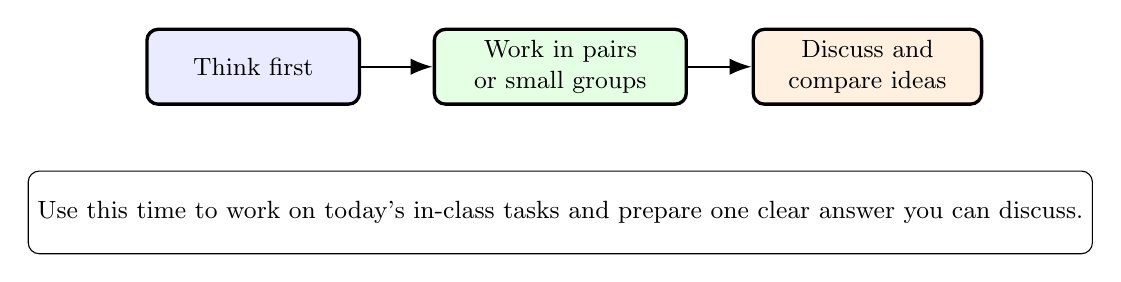
\begin{tikzpicture}[>=Latex, every node/.style={font=\small}]
    \node[draw, rounded corners, very thick, fill=blue!8, minimum width=2.7cm, minimum height=0.95cm, align=center] (think) at (-3.9,0.9) {Think first};
    \node[draw, rounded corners, very thick, fill=green!10, minimum width=3.2cm, minimum height=0.95cm, align=center] (work) at (0,0.9) {Work in pairs\\or small groups};
    \node[draw, rounded corners, very thick, fill=orange!12, minimum width=2.9cm, minimum height=0.95cm, align=center] (share) at (3.9,0.9) {Discuss and\\compare ideas};
    \draw[-{Latex[length=2.8mm]}, thick] (think) -- (work);
    \draw[-{Latex[length=2.8mm]}, thick] (work) -- (share);
    \node[draw, rounded corners, fill=white, minimum width=9.4cm, minimum height=1.05cm, align=center] at (0,-0.95) {Use this time to work on today's in-class tasks and prepare one clear answer you can discuss.};
  \end{tikzpicture}
  \end{center}
  \plainidea{#1}
}

\usetikzlibrary{positioning,arrows.meta,calc,shapes.geometric}

% -------------------------
% Theme
% -------------------------
\usetheme{Madrid}
\usecolortheme{default}
\setbeamertemplate{navigation symbols}{}

% -------------------------
% Per-slide reference footer
% -------------------------
\newcommand{\defaultdeckrefs}{AIMA4e Ch.17--18; Poole3e Ch.12--14}
\newcommand{\currentsliderefs}{\defaultdeckrefs}
\newcommand{\setslideref}[1]{\gdef\currentsliderefs{#1}}
\addtobeamertemplate{footline}{}{%
  \begin{beamercolorbox}[wd=\paperwidth,leftskip=0.4em,rightskip=0.4em,ht=2.8ex,dp=0.9ex]{author in head/foot}
    \tiny\textbf{Refs: }\currentsliderefs
  \end{beamercolorbox}
}

% -------------------------
% Metadata
% -------------------------
\title[EBU6505 B4 D5]{EBU6505 -- Reasoning and Agents\\Block 4, Day 5 -- Dynamic Decision Networks and POMDP Synthesis}
\author{Dr Riasat Islam}
\institute{Queen Mary University of London}
\date{}

% -------------------------
% TikZ styles
% -------------------------
\tikzset{
  flowarrow/.style={-{Latex[length=2.8mm]}, thick},
  chance/.style={draw, ellipse, very thick, fill=blue!10, minimum width=2.6cm, minimum height=1.0cm, align=center},
  decision/.style={draw, rounded corners=1mm, very thick, fill=green!12, minimum width=2.7cm, minimum height=1.0cm, align=center},
  utility/.style={draw, diamond, aspect=2.0, very thick, fill=orange!12, minimum width=2.8cm, minimum height=1.0cm, align=center},
  statebox/.style={draw, rounded corners, very thick, fill=blue!10, minimum width=2.3cm, minimum height=0.95cm, align=center},
  actionbox/.style={draw, rounded corners, very thick, fill=green!12, minimum width=2.3cm, minimum height=0.95cm, align=center},
  rewardbox/.style={draw, rounded corners, very thick, fill=orange!12, minimum width=2.4cm, minimum height=0.95cm, align=center},
  beliefbox/.style={draw, rounded corners, very thick, fill=purple!10, minimum width=2.5cm, minimum height=0.95cm, align=center},
  obsbox/.style={draw, rounded corners, very thick, fill=teal!10, minimum width=2.4cm, minimum height=0.95cm, align=center},
  softbox/.style={draw, rounded corners, fill=white, minimum width=2.8cm, minimum height=0.95cm, align=center},
  note/.style={draw, rounded corners, fill=white, minimum width=2.8cm, minimum height=0.85cm, align=center, font=\small}
}

\begin{document}

\setslideref{AIMA4e Ch.17--18; Poole3e Ch.12--14}
\begin{frame}
  \titlepage
\end{frame}

\begin{frame}{What have we covered this week?}
\begin{itemize}
  \item Day 1: Bayesian networks for static uncertain reasoning
  \item Day 2: exact inference in Bayesian networks
  \item Day 3: temporal models such as hidden Markov models (HMMs) and dynamic Bayesian networks (DBNs)
  \item Day 4: planning with uncertainty using utility and Markov decision process (MDP) ideas
\end{itemize}
\plainidea{This week moved from uncertain belief, to temporal belief, and then to action under uncertainty.}
\end{frame}

\begin{frame}{What are we going to cover today?}
\begin{itemize}
  \item how a dynamic decision network (DDN) adds decisions and utilities to a temporal graph
  \item what a partially observable Markov decision process (POMDP) adds when the true state is hidden
  \item how belief updates support action selection
  \item how to choose between a Bayesian network, dynamic Bayesian network, Markov decision process, dynamic decision network, and POMDP
  \item one simple healthcare case plus other domain examples
\end{itemize}
\plainidea{Today is a synthesis lecture. The goal is to connect all the models, not to add many new symbols.}
\end{frame}

\begin{frame}{Resources}
\begin{itemize}
  \item \textit{Artificial Intelligence: A Modern Approach}, 4th ed.\\
  Chapter 17: Making Complex Decisions\\
  Chapter 18: Probabilistic Reasoning over Time
  \item \textit{Artificial Intelligence: Foundations of Computational Agents}, 3rd ed.\\
  Chapter 12: Planning with Uncertainty\\
  Chapter 13: Probabilistic Inference
\end{itemize}
\plainidea{Use the AIMA reading for dynamic decision network and POMDP language, and the Poole reading for planning under uncertainty.}
\end{frame}

\begin{frame}{Learning Outcomes for Today}
By the end of this session, you should be able to:
\begin{itemize}
  \item explain how a dynamic decision network (DDN) extends a temporal probabilistic model with decisions and utilities
  \item explain the parts of a partially observable Markov decision process (POMDP) in simple language
  \item describe how action, observation, and belief fit together
  \item choose a suitable model for a simple uncertain decision problem
  \item explain one end-to-end example from sensing to action
\end{itemize}
\end{frame}

\begin{frame}{Why Do We Need One Synthesis Model?}
\keyquestion{Why are Bayesian networks, dynamic Bayesian networks, Markov decision processes, and POMDPs usually taught together at the end?}
\begin{columns}[T,onlytextwidth]
  \begin{column}{0.48\textwidth}
    \begin{tcolorbox}[colback=plainbg,colframe=plainframe,boxrule=0.7pt,title=What we already have]
    \small uncertain facts\\
    uncertain facts over time\\
    actions and utilities
    \end{tcolorbox}
    \begin{tcolorbox}[colback=questionbg,colframe=questionframe,boxrule=0.7pt,title=What we still need]
    \small one model for hidden state, observations, actions, and utility
    \end{tcolorbox}
  \end{column}
  \begin{column}{0.46\textwidth}
    \begin{center}
    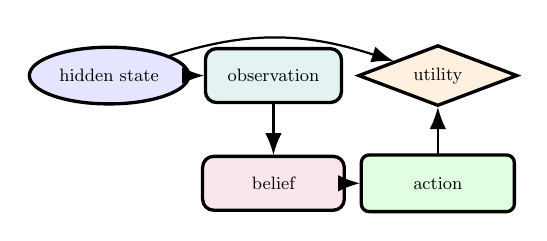
\begin{tikzpicture}[>=Latex, scale=0.72, every node/.style={font=\small, transform shape}]
      \node[chance] (h) at (0,1.0) {hidden state};
      \node[obsbox] (o) at (2.9,1.0) {observation};
      \node[beliefbox] (b) at (2.9,-0.9) {belief};
      \node[decision] (a) at (5.8,-0.9) {action};
      \node[utility] (u) at (5.8,1.0) {utility};
      \draw[flowarrow] (h) -- (o);
      \draw[flowarrow] (o) -- (b);
      \draw[flowarrow] (b) -- (a);
      \draw[flowarrow] (a) -- (u);
      \draw[flowarrow] (h) to[out=18,in=162] (u);
    \end{tikzpicture}
    \end{center}
  \end{column}
\end{columns}
\plainidea{Day 5 joins hidden state, observations, actions, and utility into one model.}
\end{frame}

\begin{frame}{Concept Map: How the Models Connect}
\keyquestion{How do Bayesian networks, DBNs, MDPs, DDNs, and POMDPs connect?}
\begin{center}
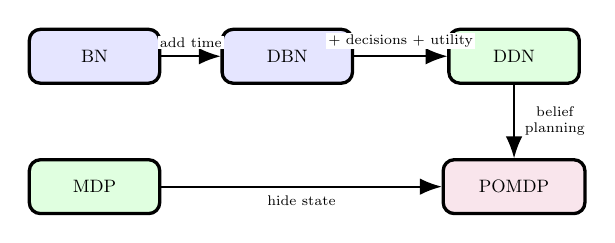
\begin{tikzpicture}[>=Latex, scale=0.72, every node/.style={font=\small, transform shape}]
  \node[statebox] (bn) at (0,1.1) {BN};
  \node[statebox] (dbn) at (3.4,1.1) {DBN};
  \node[actionbox] (ddn) at (7.4,1.1) {DDN};
  \node[actionbox] (mdp) at (0,-1.2) {MDP};
  \node[beliefbox] (pomdp) at (7.4,-1.2) {POMDP};
  \draw[flowarrow] (bn) -- node[midway, above=3pt, fill=white, inner sep=1pt, font=\scriptsize] {add time} (dbn);
  \draw[flowarrow] (dbn) -- node[midway, above=3pt, fill=white, inner sep=1pt, font=\scriptsize] {+ decisions + utility} (ddn);
  \draw[flowarrow] (mdp) -- node[midway, below=3pt, fill=white, inner sep=1pt, font=\scriptsize] {hide state} (pomdp);
  \draw[flowarrow] (ddn) -- node[midway, right=4pt, fill=white, inner sep=1pt, font=\scriptsize, align=center] {belief\\planning} (pomdp);
\end{tikzpicture}
\end{center}
\vspace{-0.3em}
\begin{columns}[T,onlytextwidth]
  \begin{column}{0.48\textwidth}
    \begin{tcolorbox}[colback=plainbg,colframe=plainframe,boxrule=0.7pt,title=Simple reading]
    \small BNs and DBNs model belief.
    \end{tcolorbox}
  \end{column}
  \begin{column}{0.48\textwidth}
    \begin{tcolorbox}[colback=questionbg,colframe=questionframe,boxrule=0.7pt,title=Simple reading]
    \small MDPs, DDNs, and POMDPs add action.
    \end{tcolorbox}
  \end{column}
\end{columns}
\plainidea{DDNs and POMDPs bring time, uncertainty, and action together.}
\end{frame}

\begin{frame}{What Is a Dynamic Decision Network?}
\keyquestion{What does a dynamic decision network add to an ordinary temporal probabilistic graph?}
\begin{columns}[T,onlytextwidth]
  \begin{column}{0.50\textwidth}
    \begin{tcolorbox}[colback=plainbg,colframe=plainframe,boxrule=0.7pt,title=DDN idea]
    \small
    Start from a DBN.\\
    Keep the time slices.\\
    Add one decision node and one utility node.
    \end{tcolorbox}
    \begin{tcolorbox}[colback=questionbg,colframe=questionframe,boxrule=0.7pt,title=Why useful?]
    \small
    Now the model says both what may happen and which action is better.
    \end{tcolorbox}
  \end{column}
  \begin{column}{0.44\textwidth}
    \begin{center}
    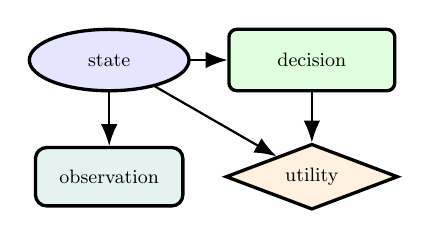
\begin{tikzpicture}[>=Latex, scale=0.78, every node/.style={font=\small, transform shape}]
      \node[chance] (s) at (0,1.0) {state};
      \node[decision] (a) at (3.3,1.0) {decision};
      \node[obsbox] (o) at (0,-0.9) {observation};
      \node[utility] (u) at (3.3,-0.9) {utility};
      \draw[flowarrow] (s) -- (a);
      \draw[flowarrow] (s) -- (o);
      \draw[flowarrow] (s) -- (u);
      \draw[flowarrow] (a) -- (u);
    \end{tikzpicture}
    \end{center}
  \end{column}
\end{columns}
\plainidea{A DDN is a temporal uncertainty model with choices and consequences added.}
\end{frame}

\begin{frame}{Two-Slice DDN Template}
\keyquestion{What does one step of a DDN usually look like?}
\begin{center}
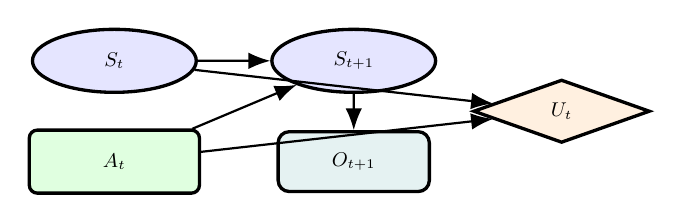
\begin{tikzpicture}[>=Latex, scale=0.80, every node/.style={font=\small, transform shape}]
  \node[chance] (s0) at (0,1.4) {$S_t$};
  \node[decision] (a0) at (0,-0.2) {$A_t$};
  \node[chance] (s1) at (3.8,1.4) {$S_{t+1}$};
  \node[obsbox] (o1) at (3.8,-0.2) {$O_{t+1}$};
  \node[utility] (u0) at (7.1,0.6) {$U_t$};
  \draw[flowarrow] (s0) -- (s1);
  \draw[flowarrow] (a0) -- (s1);
  \draw[flowarrow] (s1) -- (o1);
  \draw[flowarrow] (s0) -- (u0);
  \draw[flowarrow] (a0) -- (u0);
\end{tikzpicture}
\end{center}
\notationblock{\small $S_t$: state now, $A_t$: action now, $S_{t+1}$: next state\\
$O_{t+1}$: next observation, $U_t$: utility for this choice}
\plainidea{A dynamic decision network shows how current state and action affect the next state, the next observation, and the utility.}
\end{frame}

\begin{frame}{What Do the DDN Arrows Mean?}
\keyquestion{What kind of influence does each arrow in a DDN represent?}
\begin{columns}[T,onlytextwidth]
  \begin{column}{0.50\textwidth}
    \begin{tcolorbox}[colback=plainbg,colframe=plainframe,boxrule=0.7pt,title=Arrow meanings]
    \small
    state $\rightarrow$ next state: world dynamics\\[0.3em]
    action $\rightarrow$ next state: the choice changes what may happen\\[0.3em]
    state + action $\rightarrow$ utility: reward depends on both
    \end{tcolorbox}
  \end{column}
  \begin{column}{0.44\textwidth}
    \begin{center}
    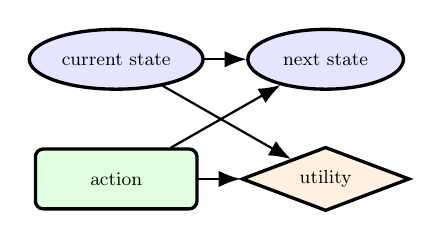
\begin{tikzpicture}[>=Latex, scale=0.76, every node/.style={font=\small, transform shape}]
      \node[chance] (s) at (0,1.1) {current state};
      \node[decision] (a) at (0,-0.9) {action};
      \node[chance] (n) at (3.5,1.1) {next state};
      \node[utility] (u) at (3.5,-0.9) {utility};
      \draw[flowarrow] (s) -- (n);
      \draw[flowarrow] (a) -- (n);
      \draw[flowarrow] (s) -- (u);
      \draw[flowarrow] (a) -- (u);
    \end{tikzpicture}
    \end{center}
  \end{column}
\end{columns}
\plainidea{The arrows show what the choice depends on and what the choice can change.}
\end{frame}

\begin{frame}{From DBN to DDN}
\keyquestion{How do we move from temporal belief tracking to temporal decision-making?}
\begin{columns}[T,onlytextwidth]
  \begin{column}{0.47\textwidth}
    \begin{tcolorbox}[colback=plainbg,colframe=plainframe,boxrule=0.7pt,title=DBN]
    hidden state over time\\
    noisy observations\\
    no explicit decision or utility
    \end{tcolorbox}
  \end{column}
  \begin{column}{0.47\textwidth}
    \begin{tcolorbox}[colback=questionbg,colframe=questionframe,boxrule=0.7pt,title=DDN]
    hidden state over time\\
    noisy observations\\
    plus decisions and utilities
    \end{tcolorbox}
  \end{column}
\end{columns}
\begin{center}
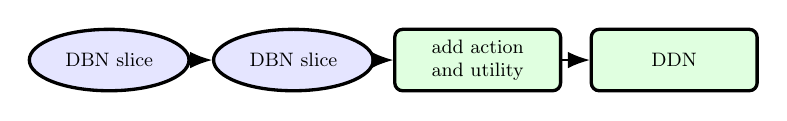
\begin{tikzpicture}[>=Latex, scale=0.78, every node/.style={font=\small, transform shape}]
  \node[chance] (dbn1) at (0,0.8) {DBN slice};
  \node[chance] (dbn2) at (3.0,0.8) {DBN slice};
  \node[decision] (add) at (6.0,0.8) {add action\\and utility};
  \node[decision] (ddn) at (9.2,0.8) {DDN};
  \draw[flowarrow] (dbn1) -- (dbn2);
  \draw[flowarrow] (dbn2) -- (add);
  \draw[flowarrow] (add) -- (ddn);
\end{tikzpicture}
\end{center}
\plainidea{A dynamic decision network is a dynamic Bayesian network plus decision-making structure.}
\end{frame}

\begin{frame}{What Is a POMDP?}
\keyquestion{What do we need when the true state is hidden but the agent must still act?}
\begin{columns}[T,onlytextwidth]
  \begin{column}{0.48\textwidth}
    \begin{tcolorbox}[colback=plainbg,colframe=plainframe,boxrule=0.7pt,title=Main challenge]
    the agent cannot directly see the true state
    \end{tcolorbox}
    \begin{tcolorbox}[colback=questionbg,colframe=questionframe,boxrule=0.7pt,title=Main solution]
    the agent plans using a belief over states instead of one known state
    \end{tcolorbox}
  \end{column}
  \begin{column}{0.46\textwidth}
    \begin{center}
    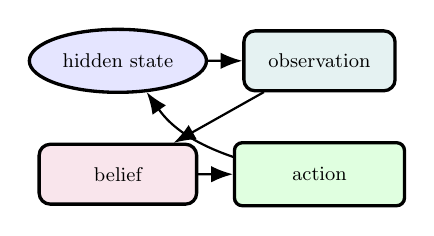
\begin{tikzpicture}[>=Latex, scale=0.80, every node/.style={font=\small, transform shape}]
      \node[chance] (s) at (0,1.0) {hidden state};
      \node[obsbox] (o) at (3.2,1.0) {observation};
      \node[beliefbox] (b) at (0,-0.8) {belief};
      \node[decision] (a) at (3.2,-0.8) {action};
      \draw[flowarrow] (s) -- (o);
      \draw[flowarrow] (o) -- (b);
      \draw[flowarrow] (b) -- (a);
      \draw[flowarrow] (a) to[bend left=18] (s);
    \end{tikzpicture}
    \end{center}
  \end{column}
\end{columns}
\plainidea{A partially observable Markov decision process (POMDP) is the standard model for sequential decisions when the world state is partly hidden.}
\end{frame}

\begin{frame}{The POMDP Pieces}
\keyquestion{What are the main pieces of a POMDP?}
\[
\mathcal{P}=(S,A,O,T,Z,R,\gamma)
\]
\begin{columns}[T,onlytextwidth]
  \begin{column}{0.48\textwidth}
    \begin{tcolorbox}[colback=notationbg,colframe=notationframe,boxrule=0.7pt,title=State and action]
    \small
    $S$: hidden states\\
    $A$: actions\\
    $O$: observations
    \end{tcolorbox}
  \end{column}
  \begin{column}{0.48\textwidth}
    \begin{tcolorbox}[colback=notationbg,colframe=notationframe,boxrule=0.7pt,title=Models and reward]
    \small
    $T$: transition model\\
    $Z$: observation model\\
    $R$: reward, $\gamma$: discount
    \end{tcolorbox}
  \end{column}
\end{columns}
\plainidea{A POMDP says how the world changes, what we can observe, and which actions are better.}
\end{frame}

\begin{frame}{Belief Update Intuition}
\keyquestion{How does the agent change its belief after acting and observing?}
\[
b_{t+1}(s')=\eta\, Z(o_{t+1}\mid s',a_t)\sum_s T(s,a_t,s')\, b_t(s)
\]
\begin{columns}[T,onlytextwidth]
  \begin{column}{0.48\textwidth}
    \begin{tcolorbox}[colback=plainbg,colframe=plainframe,boxrule=0.7pt,title=Step 1: predict]
    \small use the transition model to predict the next hidden state
    \end{tcolorbox}
  \end{column}
  \begin{column}{0.48\textwidth}
    \begin{tcolorbox}[colback=questionbg,colframe=questionframe,boxrule=0.7pt,title=Step 2: correct]
    \small use the new observation to correct that prediction
    \end{tcolorbox}
  \end{column}
\end{columns}
\begin{center}
\small
Here, $b_t(s)$ is the current belief and $\eta$ rescales the updated numbers so they sum to 1.
\end{center}
\plainidea{Belief update means: predict first, then correct with new evidence.}
\end{frame}

\begin{frame}{Action-Observation-Belief Loop}
\keyquestion{What is the repeating loop inside a POMDP?}
\begin{center}
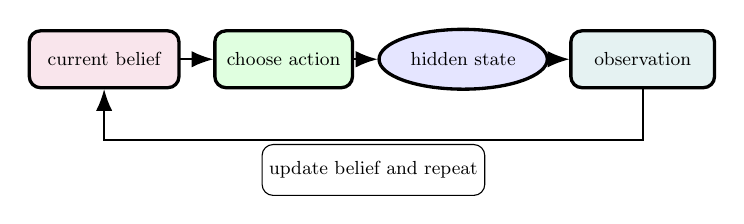
\begin{tikzpicture}[>=Latex, scale=0.76, every node/.style={font=\small, transform shape}]
  \node[beliefbox] (b) at (0,0) {current belief};
  \node[actionbox] (a) at (3.0,0) {choose action};
  \node[chance] (s) at (6.0,0) {hidden state};
  \node[obsbox] (o) at (9.0,0) {observation};
  \draw[flowarrow] (b) -- (a);
  \draw[flowarrow] (a) -- (s);
  \draw[flowarrow] (s) -- (o);
  \coordinate (loop) at (4.5,-1.35);
  \draw[flowarrow] (o.south) |- (loop) -| (b.south);
  \node[note] at (4.5,-1.85) {update belief and repeat};
\end{tikzpicture}
\end{center}
\plainidea{The agent acts, receives observations, updates belief, and then chooses again.}
\end{frame}

\begin{frame}{Mini Belief-State Example}
\keyquestion{How can one observation change the best action?}
\begin{columns}[T,onlytextwidth]
  \begin{column}{0.48\textwidth}
    \begin{tcolorbox}[colback=plainbg,colframe=plainframe,boxrule=0.7pt,title=Before warning signal]
    low risk: 70\%\\
    high risk: 30\%\\[0.3em]
    best action: continue monitoring
    \end{tcolorbox}
  \end{column}
  \begin{column}{0.48\textwidth}
    \begin{tcolorbox}[colback=questionbg,colframe=questionframe,boxrule=0.7pt,title=After warning signal]
    low risk: 35\%\\
    high risk: 65\%\\[0.3em]
    best action: alert clinician
    \end{tcolorbox}
  \end{column}
\end{columns}
\begin{center}
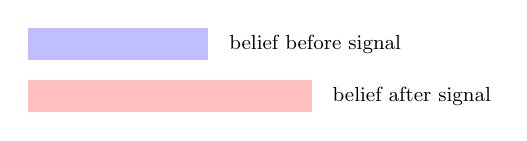
\begin{tikzpicture}[scale=0.82, every node/.style={font=\small, transform shape}]
  \fill[blue!25] (0,0) rectangle (2.8,0.5);
  \fill[red!25] (0,-0.8) rectangle (4.4,-0.3);
  \node[anchor=west] at (3.0,0.25) {belief before signal};
  \node[anchor=west] at (4.6,-0.55) {belief after signal};
\end{tikzpicture}
\end{center}
\plainidea{In a POMDP, one new observation can change the belief and therefore change the best action.}
\end{frame}

\begin{frame}{DDN Versus POMDP}
\keyquestion{What is the main difference between a DDN and a POMDP?}
\begin{center}
\begin{tabular}{>{\raggedright\arraybackslash}p{0.24\textwidth} >{\raggedright\arraybackslash}p{0.30\textwidth} >{\raggedright\arraybackslash}p{0.30\textwidth}}
\toprule
feature & DDN & POMDP \\
\midrule
main view & graphical decision model over time & sequential planning model with hidden state \\
what it emphasizes & nodes and dependencies & belief update and action choice \\
best classroom use & showing structure clearly & showing the action-belief loop clearly \\
\bottomrule
\end{tabular}
\end{center}
\plainidea{DDN and POMDP are closely related. A dynamic decision network highlights the graph structure, while a POMDP highlights belief-state planning.}
\end{frame}

\begin{frame}{One Hospital Robot Story}
\keyquestion{How do DDN and POMDP ideas appear in one simple healthcare example?}
\begin{columns}[T,onlytextwidth]
  \begin{column}{0.50\textwidth}
    \begin{tcolorbox}[colback=plainbg,colframe=plainframe,boxrule=0.7pt,title=One simple story]
    \small
    hidden part: patient risk\\[0.3em]
    evidence: noisy monitor signals\\[0.3em]
    action: continue, ask for help, or alert a clinician
    \end{tcolorbox}
  \end{column}
  \begin{column}{0.44\textwidth}
    \begin{center}
    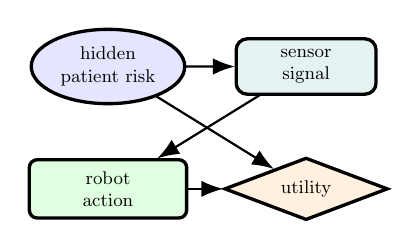
\begin{tikzpicture}[>=Latex, scale=0.74, every node/.style={font=\small, transform shape}]
      \node[chance] (risk) at (0,1.2) {hidden\\patient risk};
      \node[obsbox] (obs) at (3.4,1.2) {sensor\\signal};
      \node[decision] (act) at (0,-0.9) {robot\\action};
      \node[utility] (u) at (3.4,-0.9) {utility};
      \draw[flowarrow] (risk) -- (obs);
      \draw[flowarrow] (obs) -- (act);
      \draw[flowarrow] (risk) -- (u);
      \draw[flowarrow] (act) -- (u);
    \end{tikzpicture}
    \end{center}
  \end{column}
\end{columns}
\plainidea{The same story can be read as a DDN graph or as a POMDP planning problem.}
\end{frame}

\begin{frame}{Healthcare Decision-Support Pipeline}
\keyquestion{How does the full reasoning pipeline run from data to action?}
\begin{center}
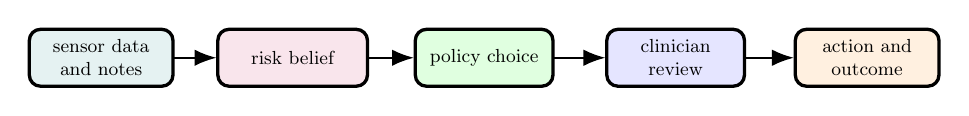
\begin{tikzpicture}[>=Latex, scale=0.76, every node/.style={font=\small, transform shape}]
  \node[obsbox] (data) at (0,0) {sensor data\\and notes};
  \node[beliefbox] (state) at (3.2,0) {risk belief};
  \node[actionbox] (policy) at (6.4,0) {policy choice};
  \node[statebox] (human) at (9.6,0) {clinician\\review};
  \node[rewardbox] (out) at (12.8,0) {action and\\outcome};
  \draw[flowarrow] (data) -- (state);
  \draw[flowarrow] (state) -- (policy);
  \draw[flowarrow] (policy) -- (human);
  \draw[flowarrow] (human) -- (out);
\end{tikzpicture}
\end{center}
\begin{columns}[T,onlytextwidth]
  \begin{column}{0.48\textwidth}
    \begin{tcolorbox}[colback=plainbg,colframe=plainframe,boxrule=0.7pt,title=Before action]
    data is used to estimate belief
    \end{tcolorbox}
  \end{column}
  \begin{column}{0.48\textwidth}
    \begin{tcolorbox}[colback=questionbg,colframe=questionframe,boxrule=0.7pt,title=At action time]
    policy and safety checks decide whether to continue, ask for review, or escalate
    \end{tcolorbox}
  \end{column}
\end{columns}
\plainidea{The model does not act on raw data directly. It acts on a belief that has already been updated.}
\end{frame}

\begin{frame}{Belief-State Policy with Safety Gates}
\keyquestion{How can one policy change its action as the risk belief changes?}
\begin{center}
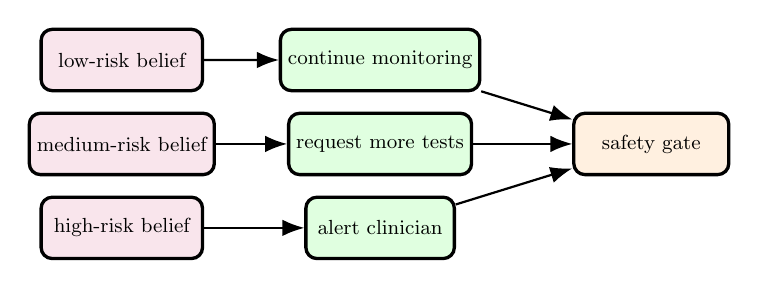
\begin{tikzpicture}[>=Latex, scale=0.82, every node/.style={font=\small, transform shape}]
  \node[beliefbox] (low) at (0,1.6) {low-risk belief};
  \node[actionbox] (a1) at (4.0,1.6) {continue monitoring};
  \node[beliefbox] (med) at (0,0.3) {medium-risk belief};
  \node[actionbox] (a2) at (4.0,0.3) {request more tests};
  \node[beliefbox] (high) at (0,-1.0) {high-risk belief};
  \node[actionbox] (a3) at (4.0,-1.0) {alert clinician};
  \node[rewardbox] (safe) at (8.2,0.3) {safety gate};
  \draw[flowarrow] (low) -- (a1);
  \draw[flowarrow] (med) -- (a2);
  \draw[flowarrow] (high) -- (a3);
  \draw[flowarrow] (a1) -- (safe);
  \draw[flowarrow] (a2) -- (safe);
  \draw[flowarrow] (a3) -- (safe);
\end{tikzpicture}
\end{center}
\plainidea{Belief guides the action, but a safety gate can still block or confirm risky choices.}
\end{frame}

\begin{frame}{What Can Go Wrong?}
\keyquestion{Why can a DDN or POMDP system still make poor decisions?}
\begin{columns}[T,onlytextwidth]
  \begin{column}{0.48\textwidth}
    \begin{tcolorbox}[colback=questionbg,colframe=questionframe,boxrule=0.7pt,title=Common problems]
    wrong transition model\\
    wrong observation model\\
    wrong utility design\\
    missing context
    \end{tcolorbox}
  \end{column}
  \begin{column}{0.48\textwidth}
    \begin{tcolorbox}[colback=plainbg,colframe=plainframe,boxrule=0.7pt,title=Why it matters]
    the system may look mathematically correct but still choose harmful or costly actions
    \end{tcolorbox}
  \end{column}
\end{columns}
\plainidea{A good algorithm is not enough. The model and the utility must also match the real task.}
\end{frame}

\begin{frame}{How Do We Reduce Risk?}
\keyquestion{What simple checks make a DDN or POMDP system safer?}
\begin{columns}[T,onlytextwidth]
  \begin{column}{0.48\textwidth}
    \begin{tcolorbox}[colback=plainbg,colframe=plainframe,boxrule=0.7pt,title=Model checks]
    calibrate sensors\\
    validate transition assumptions\\
    test utility trade-offs
    \end{tcolorbox}
  \end{column}
  \begin{column}{0.48\textwidth}
    \begin{tcolorbox}[colback=questionbg,colframe=questionframe,boxrule=0.7pt,title=Decision checks]
    keep human approval for costly actions\\
    keep a safe fallback action\\
    ask for more evidence when belief is uncertain
    \end{tcolorbox}
  \end{column}
\end{columns}
\plainidea{Safer decision-making comes from both better models and better control rules.}
\end{frame}

\begin{frame}{Which Model Should I Use?}
\keyquestion{How do I choose between BN, DBN, MDP, DDN, and POMDP?}
\small
\begin{center}
\begin{tabular}{>{\raggedright\arraybackslash}p{0.18\textwidth} >{\raggedright\arraybackslash}p{0.30\textwidth} >{\raggedright\arraybackslash}p{0.36\textwidth}}
\toprule
model & use when & key limit \\
\midrule
BN & one-time uncertain reasoning & no time and no decisions \\
DBN & temporal belief tracking & no explicit utility or action choice \\
MDP & sequential decisions with visible state & breaks when state is hidden \\
DDN & temporal decision graph with utility & still needs a clear state model \\
POMDP & sequential decisions with hidden state & harder to solve computationally \\
\bottomrule
\end{tabular}
\end{center}
\plainidea{Choose the smallest model that still matches the task structure.}
\end{frame}

\begin{frame}{Cross-Domain Map}
\keyquestion{Where do DDN and POMDP ideas appear outside healthcare?}
\begin{columns}[T,onlytextwidth]
  \begin{column}{0.48\textwidth}
    \begin{tcolorbox}[colback=plainbg,colframe=plainframe,boxrule=0.7pt,title=Autonomous driving]
    \small hidden driver intent; noisy sensing; safety actions
    \end{tcolorbox}
    \begin{tcolorbox}[colback=questionbg,colframe=questionframe,boxrule=0.7pt,title=Financial risk]
    \small hidden fraud risk; partial signals; intervention choices
    \end{tcolorbox}
  \end{column}
  \begin{column}{0.48\textwidth}
    \begin{tcolorbox}[colback=notationbg,colframe=notationframe,boxrule=0.7pt,title=Cybersecurity]
    \small hidden attack stage; noisy alerts; staged response
    \end{tcolorbox}
    \begin{tcolorbox}[colback=plainbg,colframe=plainframe,boxrule=0.7pt,title=Transport and energy]
    \small hidden demand; uncertain signals; sequential control
    \end{tcolorbox}
  \end{column}
\end{columns}
\plainidea{The same pattern appears again and again: hidden state, noisy evidence, and repeated choices.}
\end{frame}

\begin{frame}{Example: Autonomous Driving}
\keyquestion{How does hidden-state planning appear in self-driving systems?}
\begin{columns}[T,onlytextwidth]
  \begin{column}{0.48\textwidth}
    \begin{tcolorbox}[colback=plainbg,colframe=plainframe,boxrule=0.7pt,title=Hidden part]
    \small other road users may brake, turn, or cross
    \end{tcolorbox}
    \begin{tcolorbox}[colback=questionbg,colframe=questionframe,boxrule=0.7pt,title=Decision part]
    \small the car may slow down, continue, or choose a safer maneuver
    \end{tcolorbox}
  \end{column}
  \begin{column}{0.46\textwidth}
    \begin{center}
    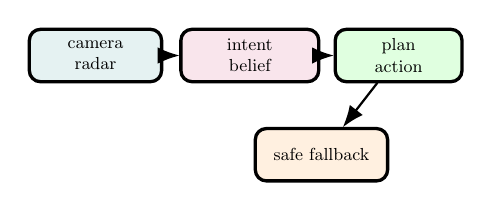
\begin{tikzpicture}[>=Latex, scale=0.70, every node/.style={font=\small, transform shape}]
      \node[obsbox] (sense) at (0,1.0) {camera\\radar};
      \node[beliefbox] (belief) at (2.8,1.0) {intent\\belief};
      \node[actionbox] (plan) at (5.5,1.0) {plan\\action};
      \node[rewardbox] (safe) at (4.1,-0.8) {safe fallback};
      \draw[flowarrow] (sense) -- (belief);
      \draw[flowarrow] (belief) -- (plan);
      \draw[flowarrow] (plan) -- (safe);
    \end{tikzpicture}
    \end{center}
  \end{column}
\end{columns}
\plainidea{Driving needs both prediction and safe action under uncertainty.}
\end{frame}

\begin{frame}{Example: Finance and Cybersecurity}
\keyquestion{What do finance and cybersecurity have in common with POMDP thinking?}
\begin{columns}[T,onlytextwidth]
  \begin{column}{0.48\textwidth}
    \begin{tcolorbox}[colback=plainbg,colframe=plainframe,boxrule=0.7pt,title=Finance]
    hidden fraud risk\\
    partial account signals\\
    actions such as allow, flag, or freeze
    \end{tcolorbox}
  \end{column}
  \begin{column}{0.48\textwidth}
    \begin{tcolorbox}[colback=questionbg,colframe=questionframe,boxrule=0.7pt,title=Cybersecurity]
    hidden attack stage\\
    noisy alert streams\\
    actions such as monitor, isolate, or escalate
    \end{tcolorbox}
  \end{column}
\end{columns}
\plainidea{Both domains require repeated action under hidden risk, not just one-time classification.}
\end{frame}

\begin{frame}{In-Class Exercises}
\exercisebreakcontent{Use the exercise time to connect hidden state, evidence, belief, action, and utility in one clear explanation.}
\end{frame}

\begin{frame}{Summary}
\begin{itemize}
  \item a DDN adds decisions and utilities to a temporal probabilistic graph
  \item a POMDP adds hidden state, observations, and belief-state planning
  \item belief update is the bridge between sensing and action
  \item the right model depends on time, observability, and decision needs
  \item the same pattern appears in healthcare, driving, finance, and cybersecurity
\end{itemize}
\plainidea{Day 5 closes the block by connecting uncertain reasoning, temporal reasoning, and decision-making.}
\end{frame}

\begin{frame}{Block 4 Close-Out}
\begin{itemize}
  \item belief under uncertainty: Bayesian networks
  \item temporal belief: HMMs and DBNs
  \item visible-state planning: MDP ideas
  \item hidden-state planning: DDN and POMDP synthesis
  \item next step: apply the right model to your own scenario
\end{itemize}
\plainidea{Block 4 gives you one complete arc from uncertain evidence to informed action.}
\end{frame}

\begin{frame}{Further Study}
\begin{itemize}
  \item Read Poole Chapters 12--13 and revisit AIMA Chapters 17--18.
  \item Practice: Poole Ch.12, Exercises 12.13, 12.15, 12.16, 12.17, and 12.18.
  \item AIMA complex-decisions exercise page: 17.15, 17.16, and 17.17.
  \item AIMA probabilistic-reasoning-over-time exercise page: 15.15, 15.17, and 15.18.
  \item Focus on belief-state update, partially observed action choice, and how hidden-state planning differs from standard Markov decision process planning.
\end{itemize}
\end{frame}

\end{document}
